\section{Introduction}
\label{sec:introduction}

\begin{frame}{Why are we here?}
  \pause
  \begin{itemize}
    \item Probably because I asked you to come.
  \end{itemize}
\end{frame}

\begin{frame}{Why are we here?}
  \begin{itemize}
    \item {\huge Model a nuclear reactor.}
      \pause
      \begin{itemize}
        \item Neutron distribution.
        \item Thermal Hydraulics.
        \item Thermal Expansion.
      \end{itemize}
  \end{itemize}
\end{frame}

\begin{frame}{But they did it in the 1960s!}
  \begin{itemize}
    \item You're right.
    \item Computers are different now.
    \item Mathematical methods are more efficient now.
    \item \textbf{FORTRAN} has \textit{a few} new standards.
  \end{itemize}
\end{frame}

\begin{frame}{Goals}
  \begin{itemize}
    \item User input.
      \begin{itemize}
        \item Reactor geometry via \texttt{VTK} mesh.
        \item Temperature dependent cross-sections either plain-text or 
          \texttt{ISOTXS}.
        \item Pin dimensions and material compositions.
      \end{itemize}
    \item Simulate thermal expansion and thermal hydraulics internally.
    \item Collect \keff, multigroup scalar fluxes, reactor power, and average
      material temperatures.
  \end{itemize}
  %\\
  \begin{itemize}
    \item Thermal expansion and thermal hydraulic simulations have been moved
      internally and are now inherent to the simulation.
    \item Thermal hydraulic simulation also improves the accuracy of neutronics
      simulation by leading to more accurate cross sections.
  \end{itemize}
\end{frame}

\begin{frame}
  \begin{figure}
    \centering
    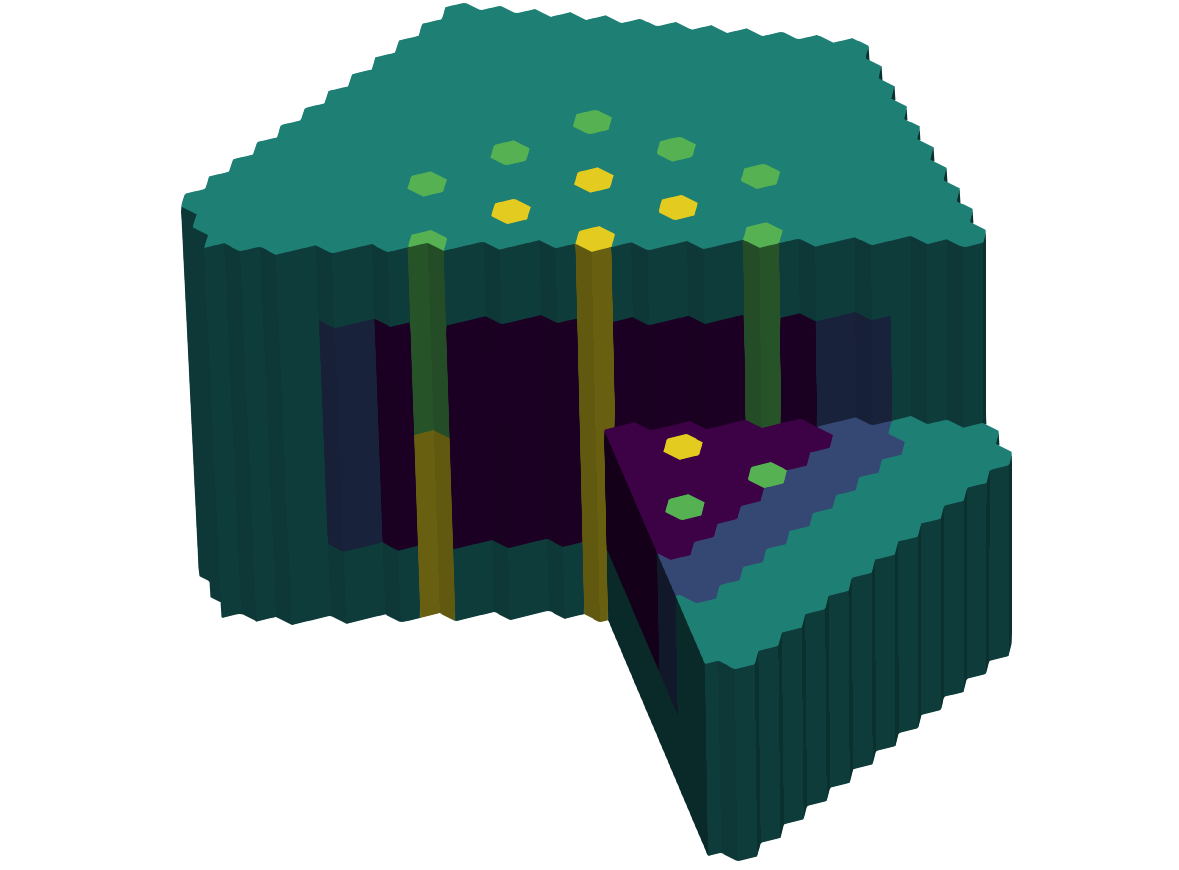
\includegraphics[width=0.9\textwidth]{reactor_materials}
    \caption{Example of Fast Reactor Materials based on MONJU.}
    \label{fig:reactor_materials}
  \end{figure}
\end{frame}

\begin{frame}
  \begin{figure}
    \centering
    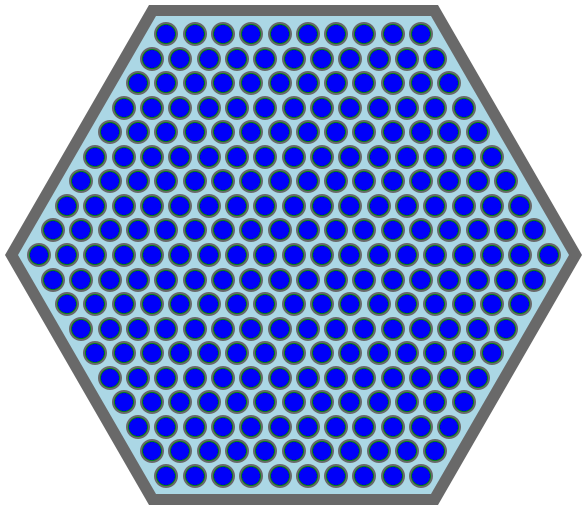
\includegraphics[width=0.5\textwidth]{prism_hex}
    \caption{Example of Fast Reactor Fuel Assembly Cross-Section.}
    \label{fig:prism_hex}
  \end{figure}
\end{frame}

\begin{frame}
  \begin{figure}
    \centering
    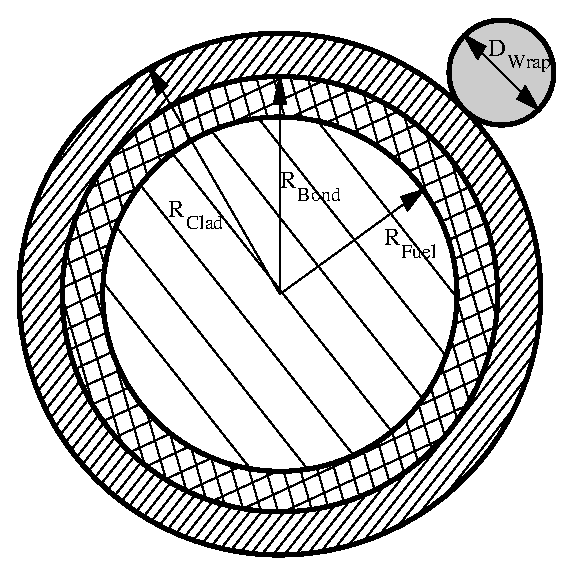
\includegraphics[width=0.5\textwidth]{pin_model}
    \caption{Dimensions of Thermal Hydraulic Rod Model.}
    \label{fig:pin_model}
  \end{figure}
\end{frame}

\begin{frame}
  \begin{figure}
    \centering
    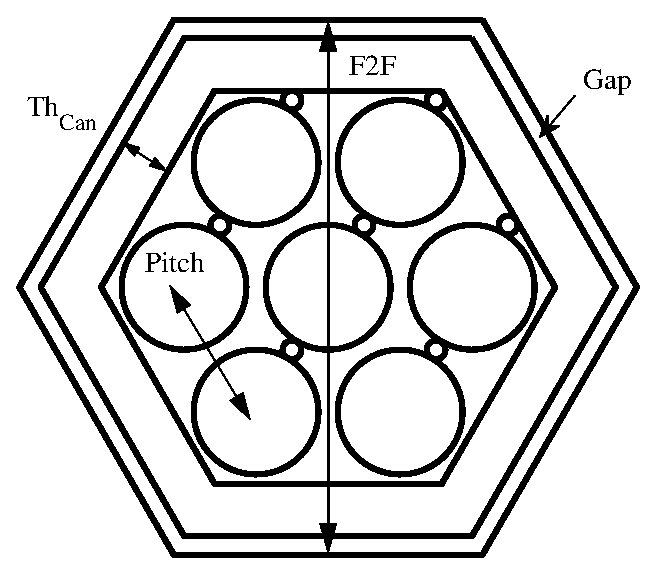
\includegraphics[width=0.5\textwidth]{hex_can}
    \caption{Dimensions of Hexagonal Can.}
    \label{fig:hex_can}
  \end{figure}
\end{frame}

